%%%%%%%%%%%%%%%%%%%%%%%%%%%%%%%%%%%%%%%%%%%%%%%%%%%%%%%%%%%%%%%%%%%%%%%
%%%%  Load the document class and packages                         %%%%
%%%%%%%%%%%%%%%%%%%%%%%%%%%%%%%%%%%%%%%%%%%%%%%%%%%%%%%%%%%%%%%%%%%%%%%
\documentclass[a4paper]{report}
\usepackage{epsfig}            % to insert PostScript figures
\graphicspath{ 
  {figures/} 
}

%Change figure names
\renewcommand{\figurename}{Fig}

\usepackage[bf,footnotesize]{caption} % make captions small and label bold


\addtocounter{chapter}{1} %Because starting at zero is silly
\makeatletter
\renewcommand{\thesection}{\@arabic\c@section}
\renewcommand{\thefigure}{\@arabic\c@figure}
\makeatother

\usepackage[a4paper,margin=2.7cm,tmargin=2.5cm,bmargin=2.5cm]{geometry} 
\usepackage{textcomp}          % To make nice degree symbols and others\usepackage[bf,footnotesize]{caption} % make captions small and label bold
\usepackage{wrapfig}
%to produce the clickable references along the left in Acroread. This
%package must be included last. 
\usepackage[ps2pdf,bookmarks=TRUE]{hyperref} 



\usepackage{wasysym}





%%%%%%%%%%%%%%%%%%%%%%%%%%%%%%%%%%%%%%%%%%%%%%%%%%%%%%%%%%%%%%%%%%%%%%%
%%%%  Hypertext references for Acrobat                             %%%%
%%%%%%%%%%%%%%%%%%%%%%%%%%%%%%%%%%%%%%%%%%%%%%%%%%%%%%%%%%%%%%%%%%%%%%%
\hypersetup{
pdfauthor = {SWC},
pdftitle = {Optics Exercises},
pdfkeywords = {optics, lenses, refraction, reflection, dispersion,
  telescope, microscope},
pdfcreator = {LaTeX with hyperref},
pdfproducer = {dvips + ps2pdf}
           }


\begin{document}




%set the number of sectioning levels 
\setcounter{secnumdepth}{2}

\begin{center}
\textbf{\Large{Optics Bench Exercises \\ \vspace{5mm} Building a brightfield microscope}}
\end{center}

\vspace{10mm}

The goal of this exercise is to build a brightfield microscope with K\"{o}hler illumination. We will do this in steps to understand the importance of illuminating the sample uniformly and from a wide range of angles. Important: think about WHY we make you place specific parts in a specific order.


\section{Critical illumination of a sample}
In critical illumination the light source is focused onto the specimen.
This provides illumination from a range of angles but has a major drawback which will become apparent soon. 

\subsection{Optical axis}
We will first create an 'optical axis' using a laser pointer - this will help us align the optics. Set the laser at one end of the rail and align the beam with the rail (horizontal and centred) using a single iris:
\begin{itemize}
    \setlength\itemsep{0.1em}
    \item Set the iris to a height suitable for adding 2'' optics. You can mount the iris to a $75~mm$ post and use a $50~mm$ post holder. 
    \item Clamp the laser pointer to one end of the rail.
    \item With the iris closest to the pointer, \textit{move/translate} the pointer until it goes through the iris. 
    \item Slide the iris to the other end of the rail and \textit{tilt} the pointer until it goes through the iris. 
    \item Repeat until the beam is parallel with the rail. 
\end{itemize} 

\begin{figure}[h]
\center
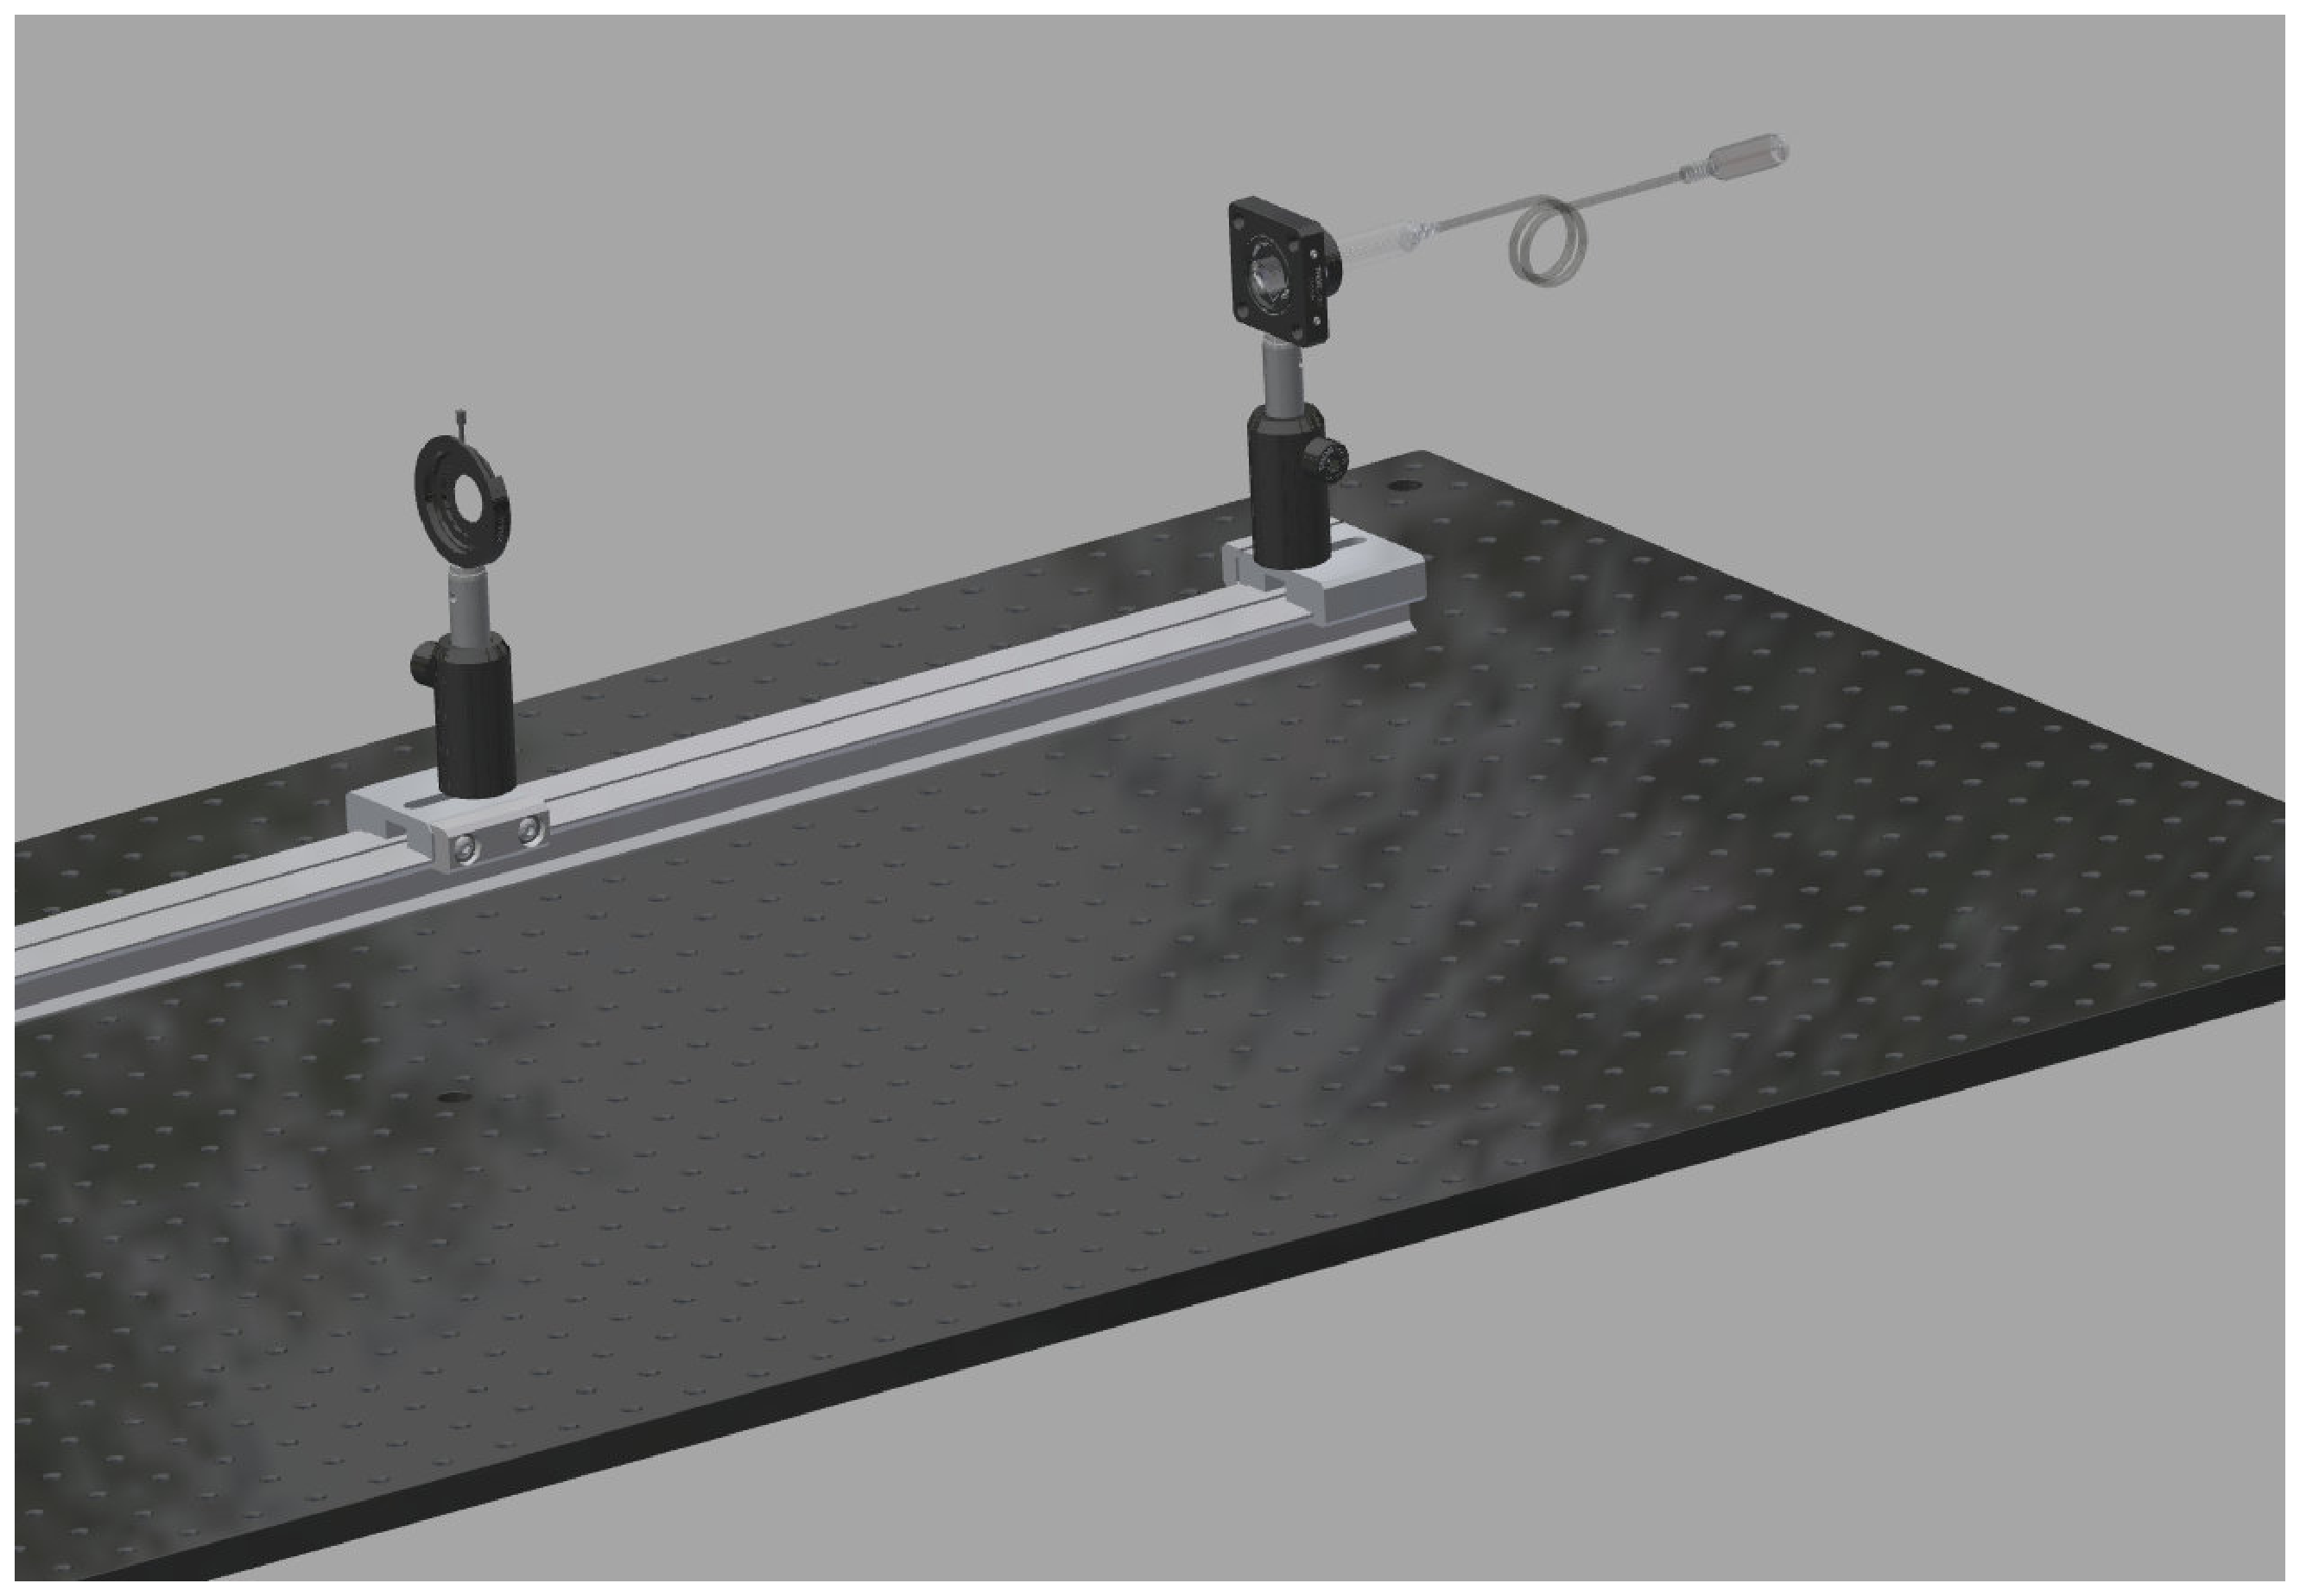
\includegraphics[width=3in]{iris_and_laser.eps}
\caption{Aligning a laser beam to the rail using an iris.}
\label{fig:beam_iris}
\end{figure}

\clearpage

\subsection{Imaging optics}
Once you're done, place a positioning collar around the iris post so you can retain its height even if you have to remove it from the post holder. We start at the end of the microscope, with the tube lens and objective (Fig.~\ref{fig:beam_obj_tube}). 

\begin{itemize}
\item Hint: In addition to the iris, use `back reflections' of the laser to align optics
\item Slide the iris to the end of the rail. 
\item Place the $f=300~mm$ lens $1f$ from the iris and adjust it until the beam goes through the iris. This is your `tube lens'.
\item Place the 4x objective before the tube lens and align it such that the beam (now expanded) again goes through the iris. What is the magnification of your imaging system?
\item Why are we starting from the back of the microscope? Why the tube lens first?
\end{itemize}

\begin{figure}[h]
\center
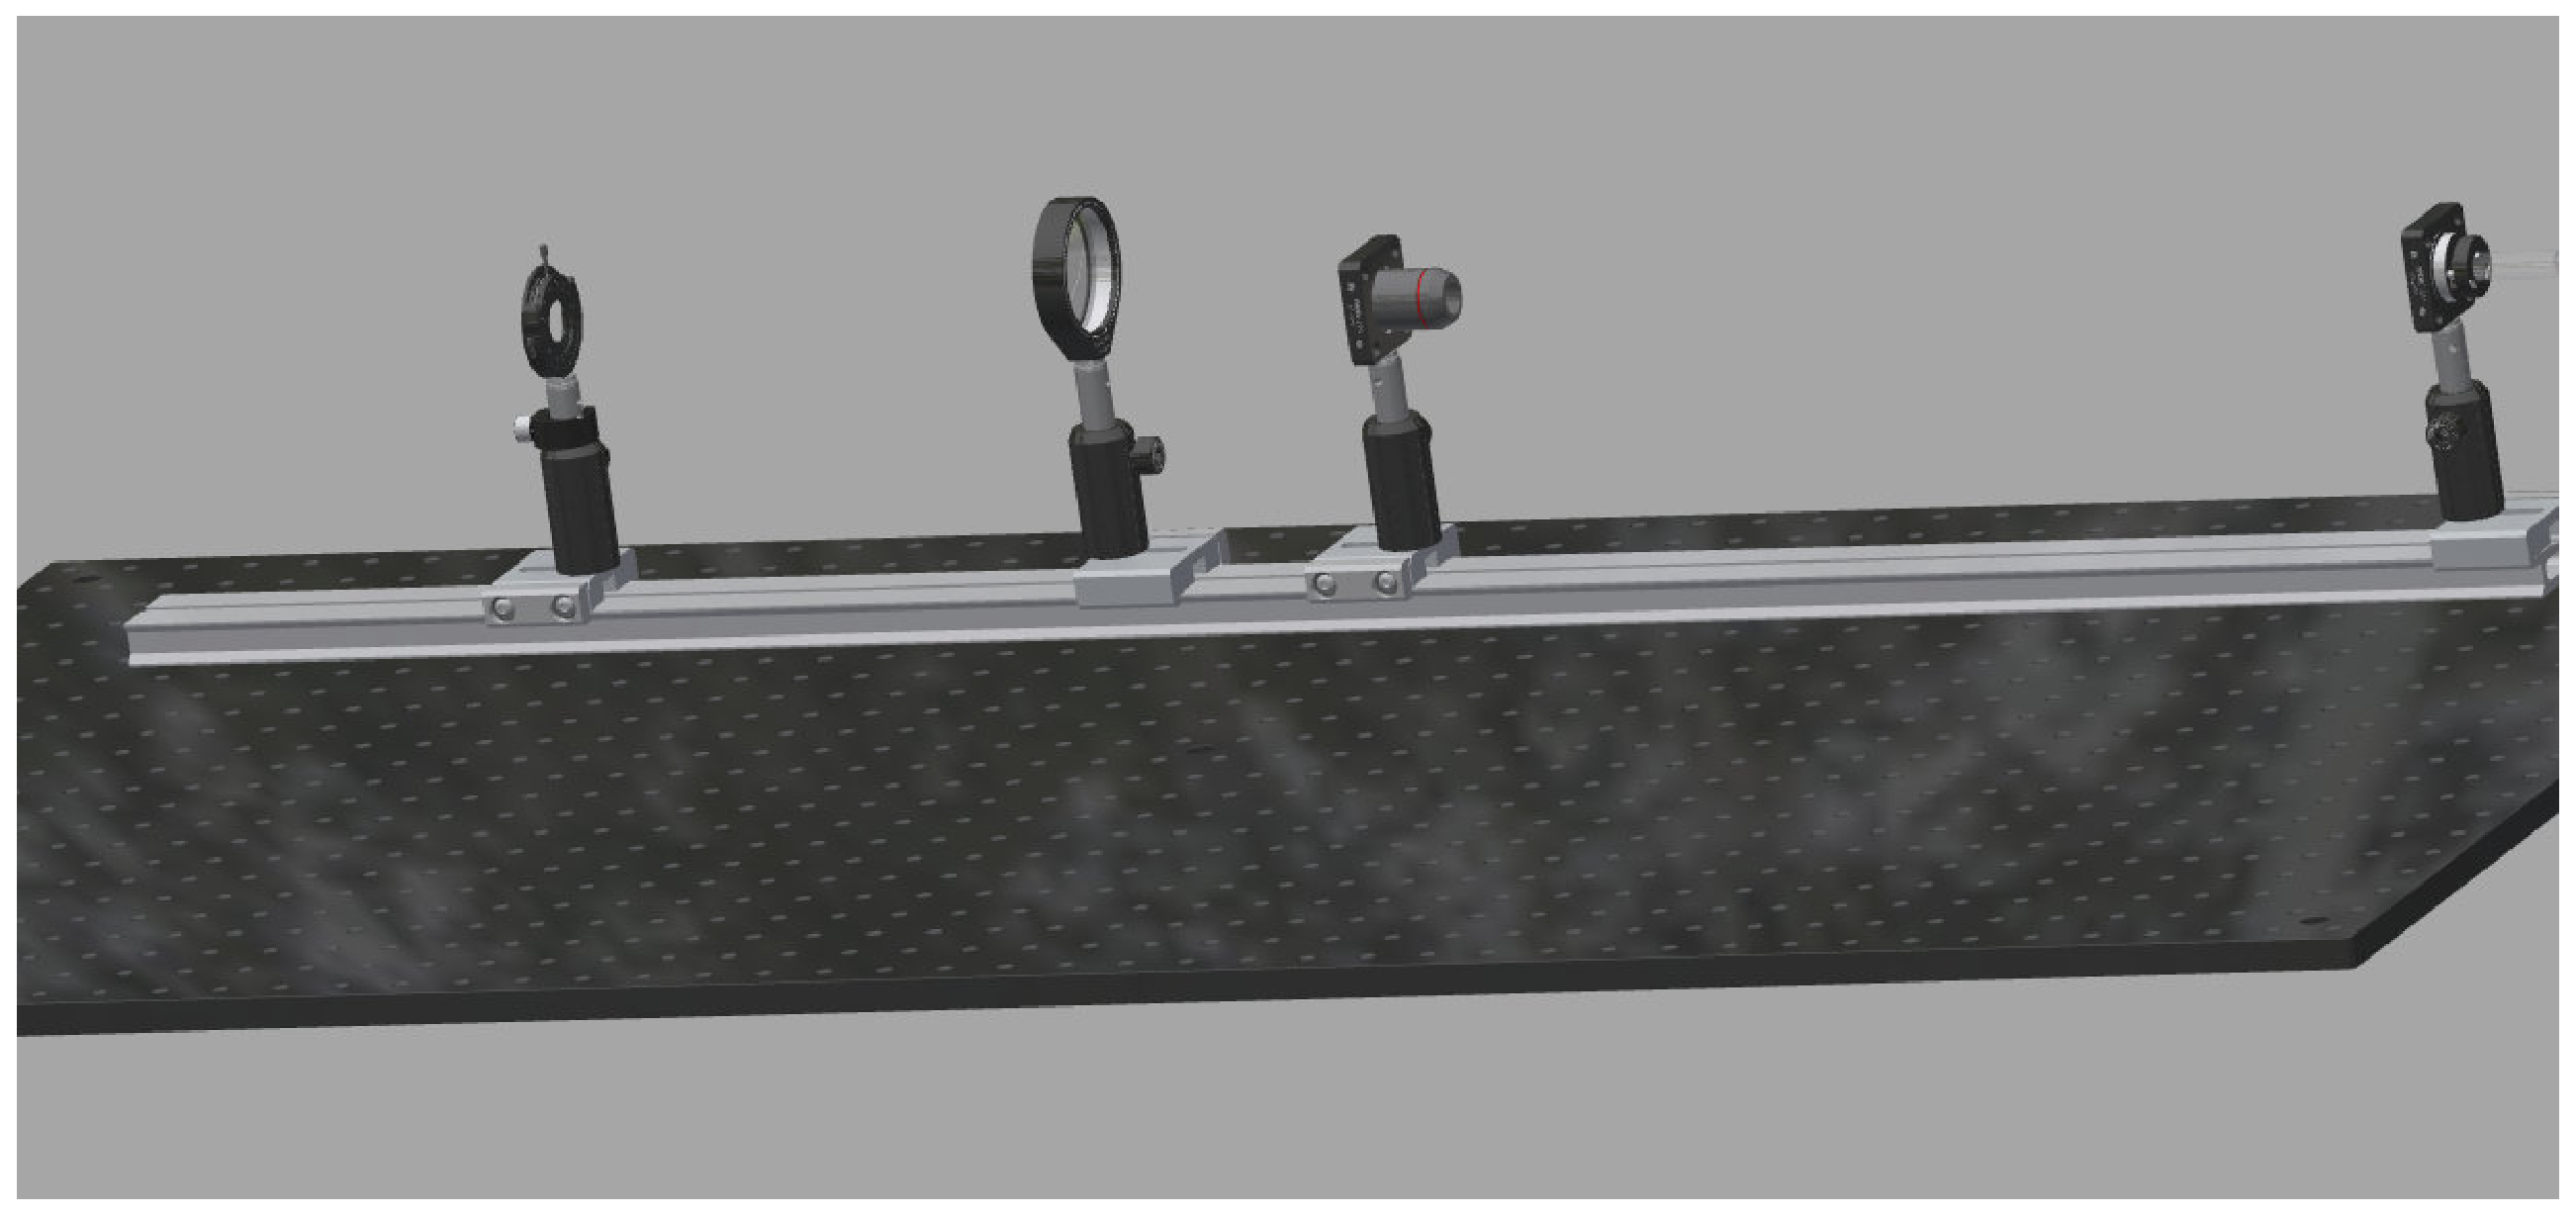
\includegraphics[width=3in]{Obj_alignment_before.eps}
\caption{Aligning the tube lens and objective with the beam.}
\label{fig:beam_obj_tube}
\end{figure}

\subsection{Basic illumination optics}
Let's place a sample and illuminate it with an LED, completing our simple microscope.

\begin{itemize}
\item Hint: Use $30~mm$ or $40~mm$ posts for the 2'' lenses, sample holder, and card holder.
\item Place your sample holder in front of the objective (about mid-rail)
\item Place the LED and choose one of the 1''{\diameter} $f=25~mm$ or $f=35~mm$ lenses to direct light onto the sample. Can you see the image of the LED? Where does the image form?
\item At the other end of the rail where the iris was, place a viewing screen onto which you will form an image - move the objective to focus.
\end{itemize}

The above arrangement is a simple microscope. How can you modify the illumination to make it brighter? Discuss with a TA and Implement it.
\\

You now have an infinite conjugate illumination system, giving you control over the illumination NA by placing an iris in the infinite space. Draw the ray diagram to predict what effect this has on the image. Test it with a sample! (Fig.~\ref{fig:critical_iris}).
\\

\subsection{Upgrade to K\"{o}hler illumination}
Discuss what is missing/wrong with your microscope. 

\begin{itemize}
	\item Use your K\"{o}hler notes to reason through this and implement the necessary changes
	\item Find ways to verify that your microscope is well aligned (optics placed in correct positions). Do you have independent control over illumination field and NA?
	\item Add the camera, check out different samples
	\item Impress a TA with your accomplishment
	\item Switch to a 10x objective - what determines how well you can image the sample? What is better compared to the 4x?
\end{itemize}

\begin{figure}[h]
\center
\includegraphics[width=2.8in]{critical_open_iris.eps}
\includegraphics[width=2.8in]{critical_closed_iris.eps}
\caption{Critical illumination with two lenses. 
There is an iris after that collector lens that is open on the left image and closed on the right image. 
Note how closing the iris restricts the range of angles reaching the sample.}
\label{fig:critical_iris}
\end{figure}

\vspace{30mm}
You have finished! Unfortunately, the princess is another castle. See you tomorrow.


\clearpage


\section{Reference: K\"{o}hler Illumination}
K\"{o}hler illumination is an important and commonly used technique in light microscopy, as it provides even illumination of the sample whilst ensuring the light source (e.g. the bulb filament) is not visible. 
This is achieved by adding a third lens, the field lens, before the condenser so that the image of the light source is out of focus at the sample. 
Since the source is out of focus, the illumination is uniform. 
Instead, the image is formed at $1f$ from the field lens. 
The condenser is then located at $1f$ from this image (as in a beam expander) so collimated (i.e. out of focus) light reaches the sample. 

The key to understanding K\"{o}hler illumination is to consider the two sets of conjugate planes in the system (Fig.~\ref{fig:koehler}). 
The \textbf{sample} is, of course, conjugate with the image plane but it also conjugate with a point $1f$ from the collector lens ($f_{CL}$ in Fig.~\ref{fig:koehler}). 
The \textbf{light source} is conjugate with a location between the field lens and the condenser ($f_F$ and $f_{CO}$ in Fig.~\ref{fig:koehler}). 
The light source is also conjugate with the objective back aperture (not shown in Fig.~\ref{fig:koehler}). 

\begin{figure}[ht]
\center
\includegraphics[width=5in]{koehler.eps}
\caption{K\"{o}hler Illumination. 
The blue lines indicate the conjugate relationship between the sample plane and the location of the field diaphragm.
The yellow lines indicate the conjugate relationship between the light source plane and the location of the aperture diaphragm.
}
\label{fig:koehler}
\end{figure}

At the two conjugate planes in the illumination path are two irises (diaphragms). 
The \textbf{field diaphragm} is at $1f$ before the field lens, in the point conjugate with the sample. 
The field lens and condenser lens form an infinite conjugate system that image the field diaphragm onto the sample. 
The field diaphragm appears in focus at the sample and is used to regulate the area of illumination. 
This helps to improve contrast by minimizing stray light. 
Remember, the The \textbf{f}ield planes are the image \textbf{f}orming planes. 

The \textbf{aperture diaphragm} is located in the plane conjugate with the light source. 
i.e. it is located where an image of the light source is formed. 
Opening and closing this diaphragm regulates which regions of the light source can contribute to the illumination. 
Closing the diaphragm blocks off-axis regions of the light source and stops them from generating the more oblique rays that come out of the condenser. 
Closing the aperture diaphragm reduces the NA of the illumination and increases depth of field. 

\clearpage

The completed arrangement of the components is shown in Fig.~\ref{fig:koehler_completed}. 
The components will be arranged in the following order and are all at $1f$ from each other (Fig.~\ref{fig:koehler}):
\begin{enumerate}
\setlength\itemsep{0.1em}
\item Collector lens
\item Field diaphragm.
\item Field lens ($f=60$)
\item Aperture diaphragm
\item Condenser lens ($f=60$)
\item The objective and tube lenses as before.
\end{enumerate}




\begin{figure}[h]
\center
\includegraphics[width=5.5in]{illum_complete.eps}
\caption{The completed K\"{o}hler illumination assembly on a rail.}
\label{fig:koehler_completed}
\end{figure}






\end{document}
